\subsection{Reconnaissance de chiffres écrits}

\begin{frame}{La base de données}
	\begin{block}{Description}
		Images de taille $28 \times 28$ pixels en noir et blanc : \\
		\quad - 60 000 images pour l'entrainement. \\
		\quad - 10 000 autres pour la vérification.
	\end{block}
	\begin{figure}
		\centering
		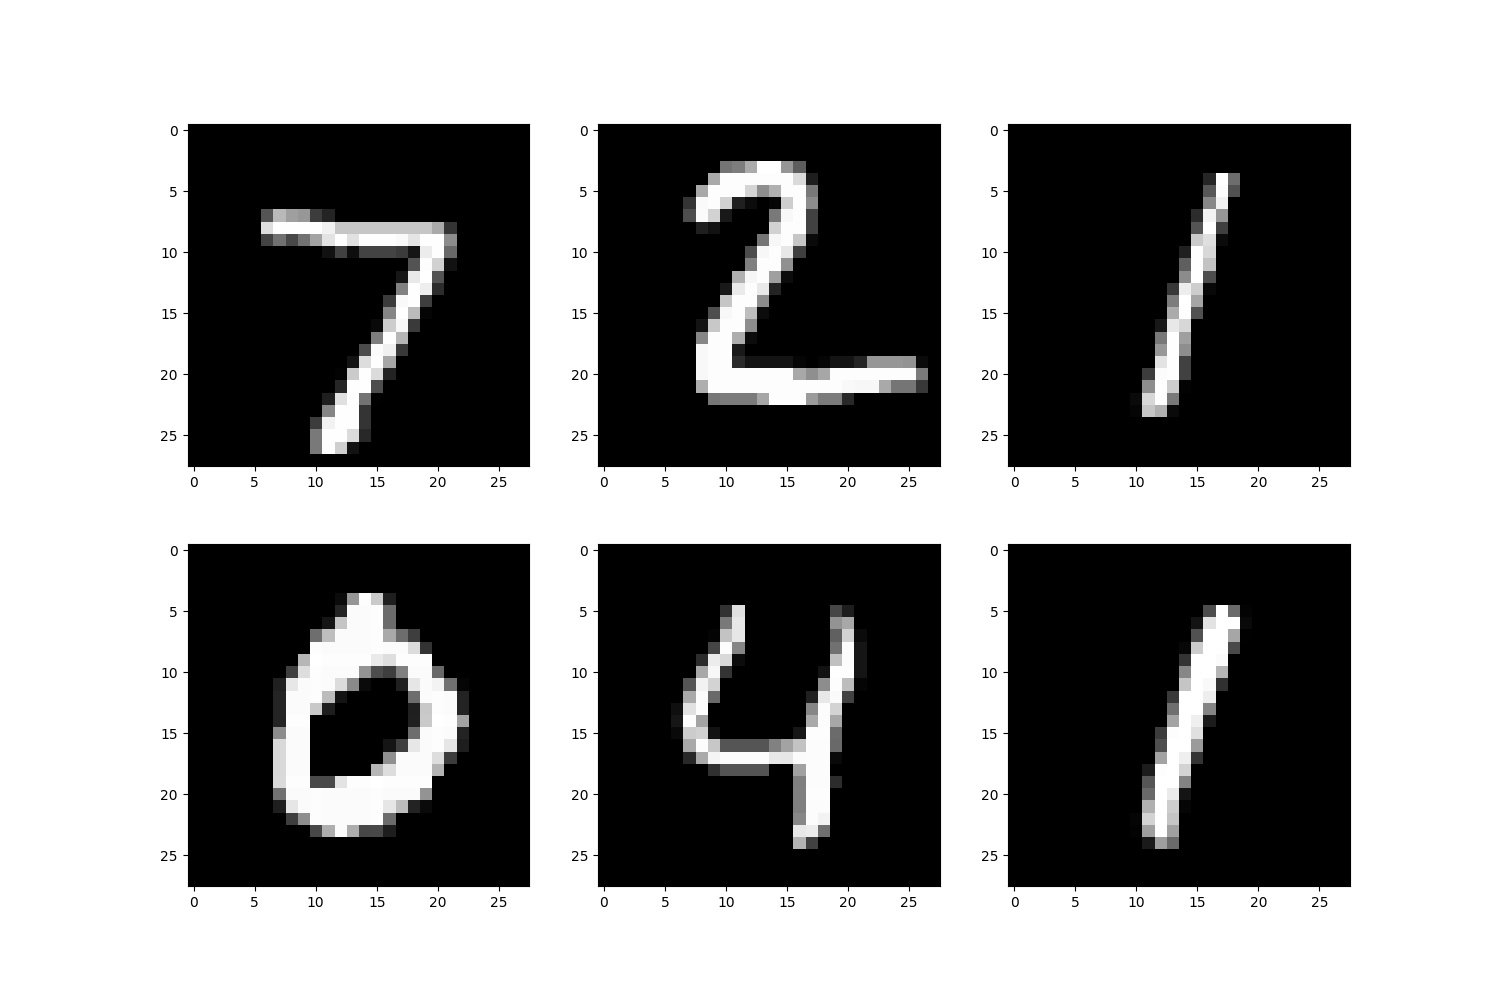
\includegraphics[width=150px]{1-mnist.jpg}
		\caption{Exemple d'images}
	\end{figure}
\end{frame}


\begin{frame}{Un réseau de neurones pour la classification}
	\begin{block}{Softmax}
		La fonction d'activation softmax permet d'obtenir en sortie une distribution de probabilité : \\
		• $p_i = \frac{exp(a_i)}{\sum_{k=1}^{n}exp(a_k)}$ la probabilité de la sortie $a_i$ \\
		• $\dfrac{\partial p_i}{\partial a_j} = p_i\times(\delta_{ij}-p_j)$ \\
	\end{block}
\end{frame}



\begin{frame}{L'utilisation de la fonction Softmax}
	\begin{figure}
		\centering
		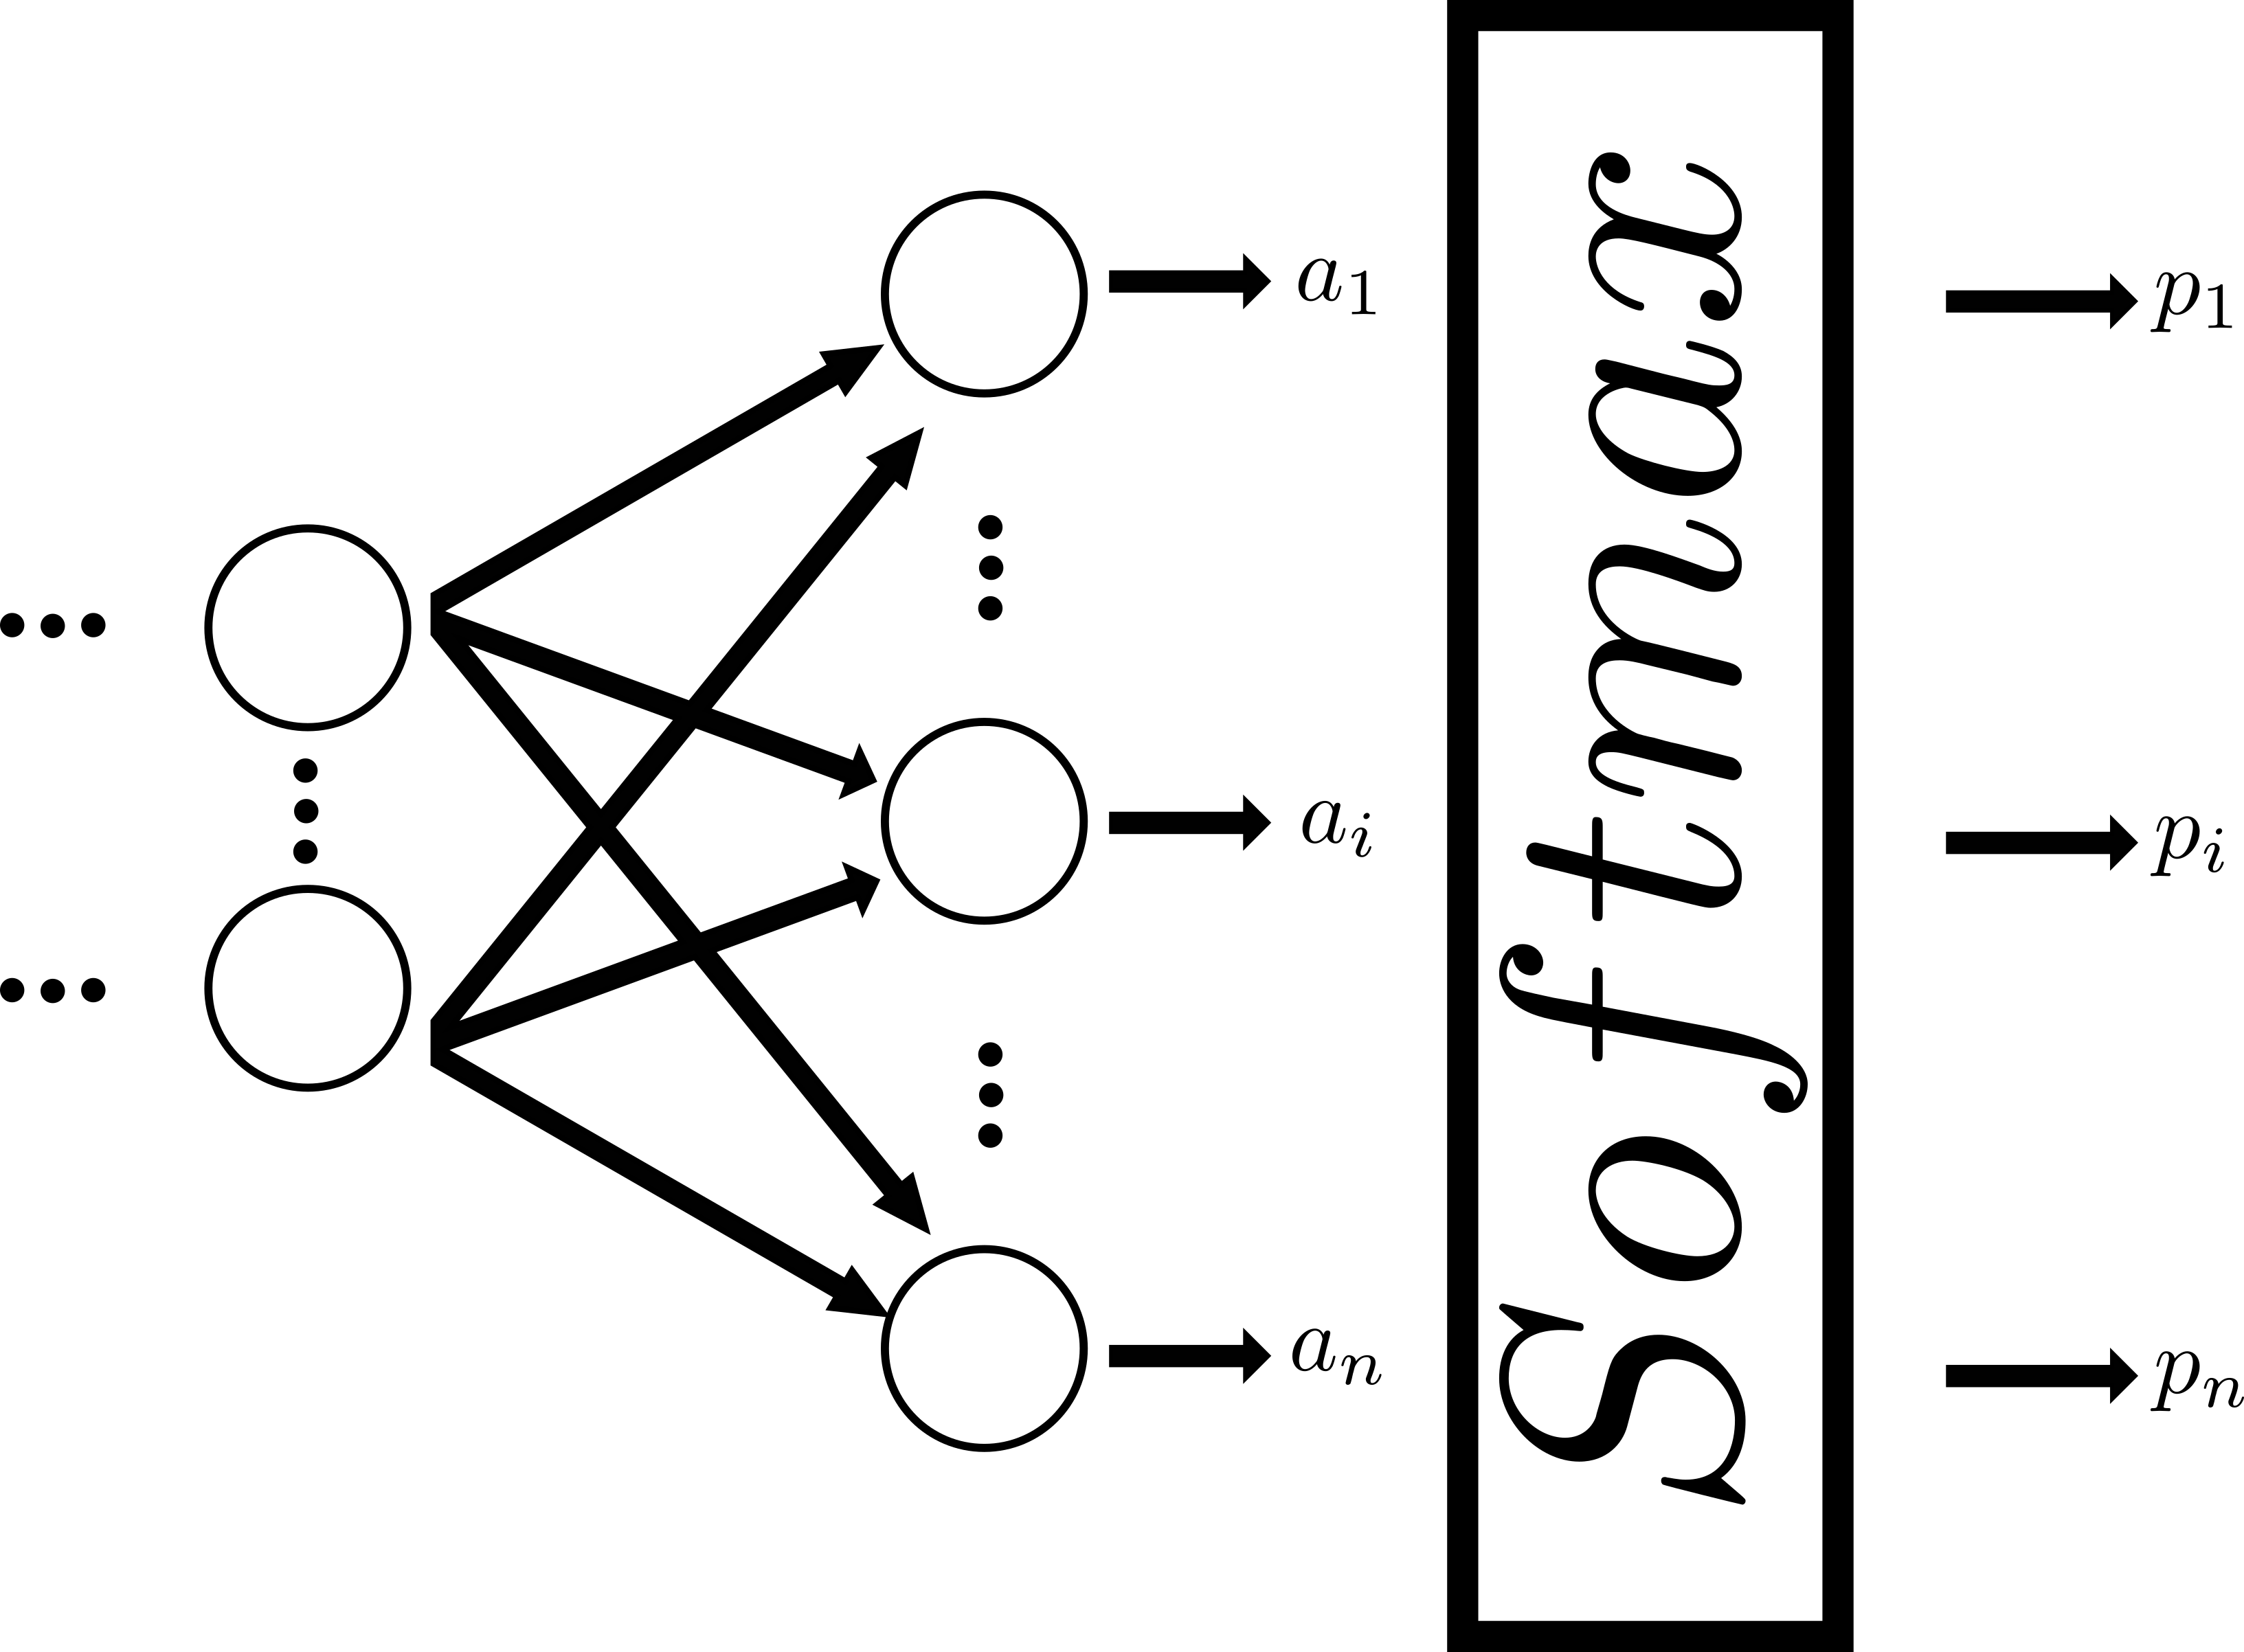
\includegraphics[height=150px]{2-Softmax.png}
		\caption{Schéma d'utilisation du Softmax}
	\end{figure}
\end{frame}


\begin{frame}{La rétropropagation pour la classification}
	\begin{block}{Cross-entropy}
		La fonction d'erreur des problèmes de classification est Cross-entropy : \\
		• $L\ \ \ = -\sum_{k=1}^{n}y_ilog(p_i)$ avec $y_i$ la sortie attendue \\
		• $\dfrac{\partial L}{\partial a_i} = p_i - y_i$
	\end{block}

\end{frame}

\begin{frame}{L'évolution de l'apprentissage}
	\begin{columns}[T] % align columns
		\begin{column}{.58\textwidth}
			\begin{figure}
				\centering
				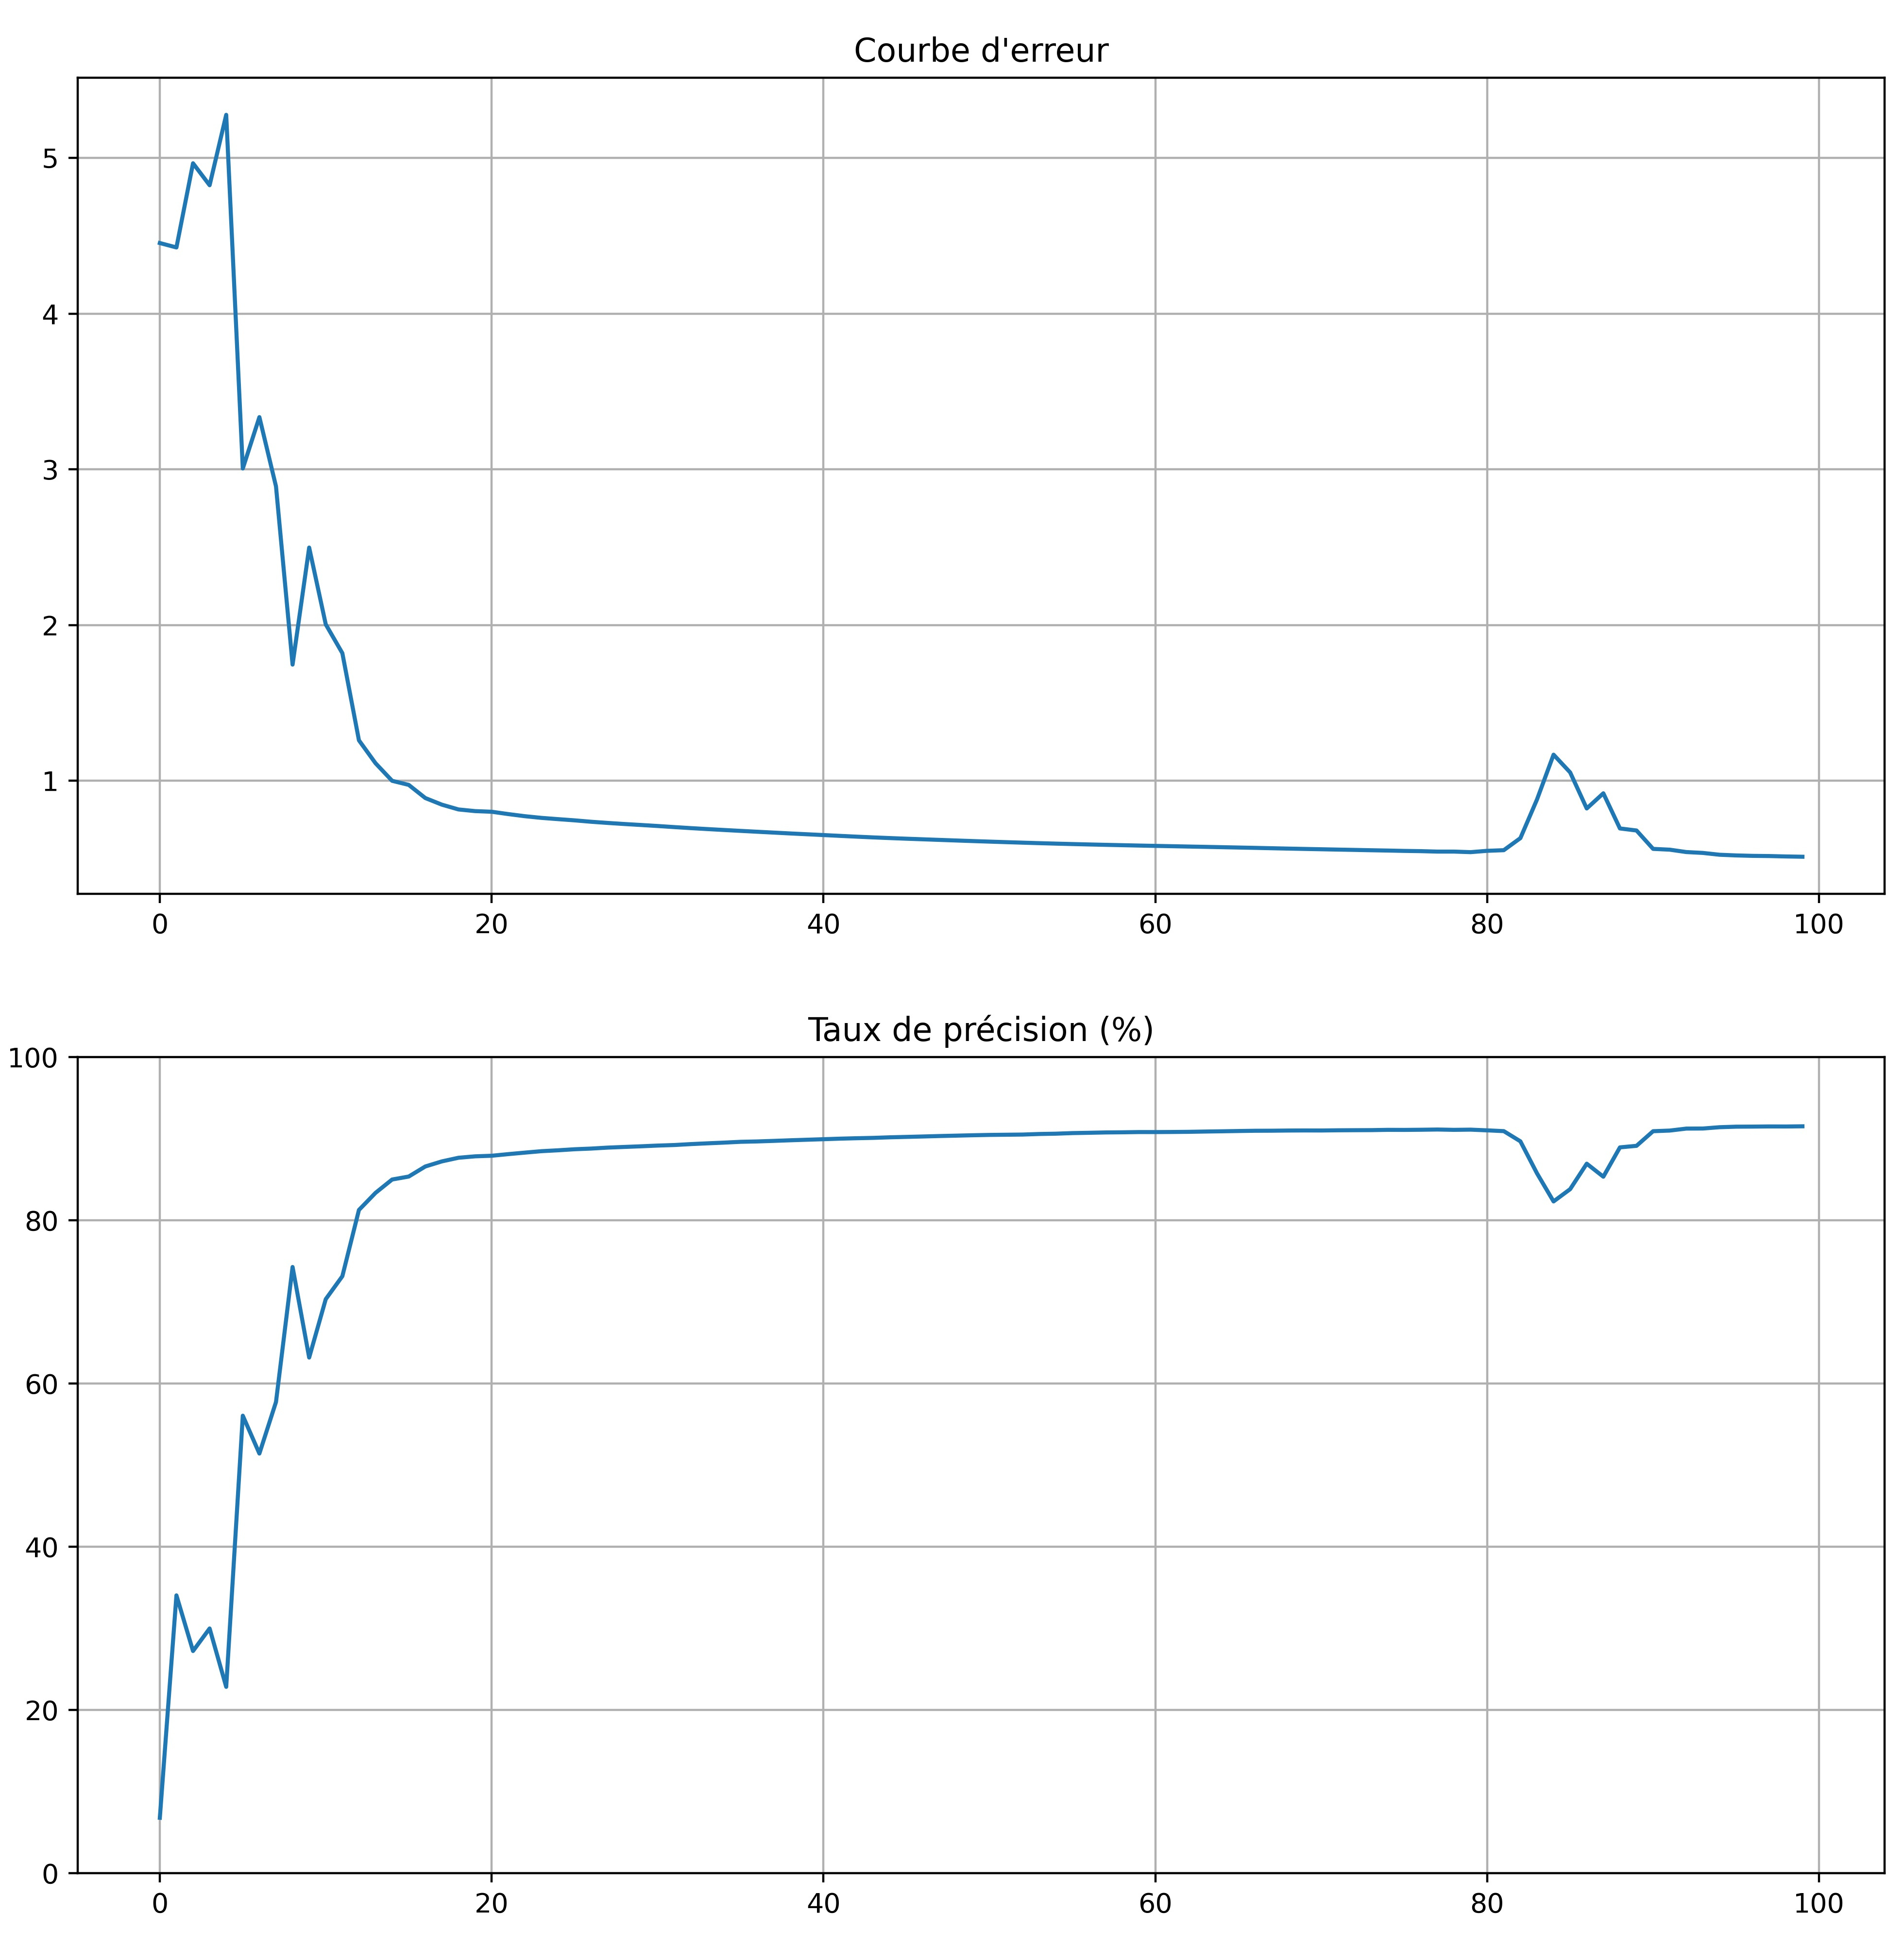
\includegraphics[height=0.7\textheight]{3-Apprentissage.jpg}
				\caption{Courbes d'apprentissage}
			\end{figure}
		\end{column}
		\hfill
		\begin{column}{.54\textwidth}
			\bigskip	\bigskip	\bigskip
			\bigskip	\bigskip	\bigskip
			\bigskip	\bigskip	\bigskip
			Taux de bonnes réponses après 100 générations d'entrainement : \\
			- 91.5\% sur les données d'entrainement \\
			- 91.3\% sur les données de validation. \\
		\end{column}%
	\end{columns}
\end{frame}


\begin{frame}{Mes résultats}
	\begin{figure}
		\centering
		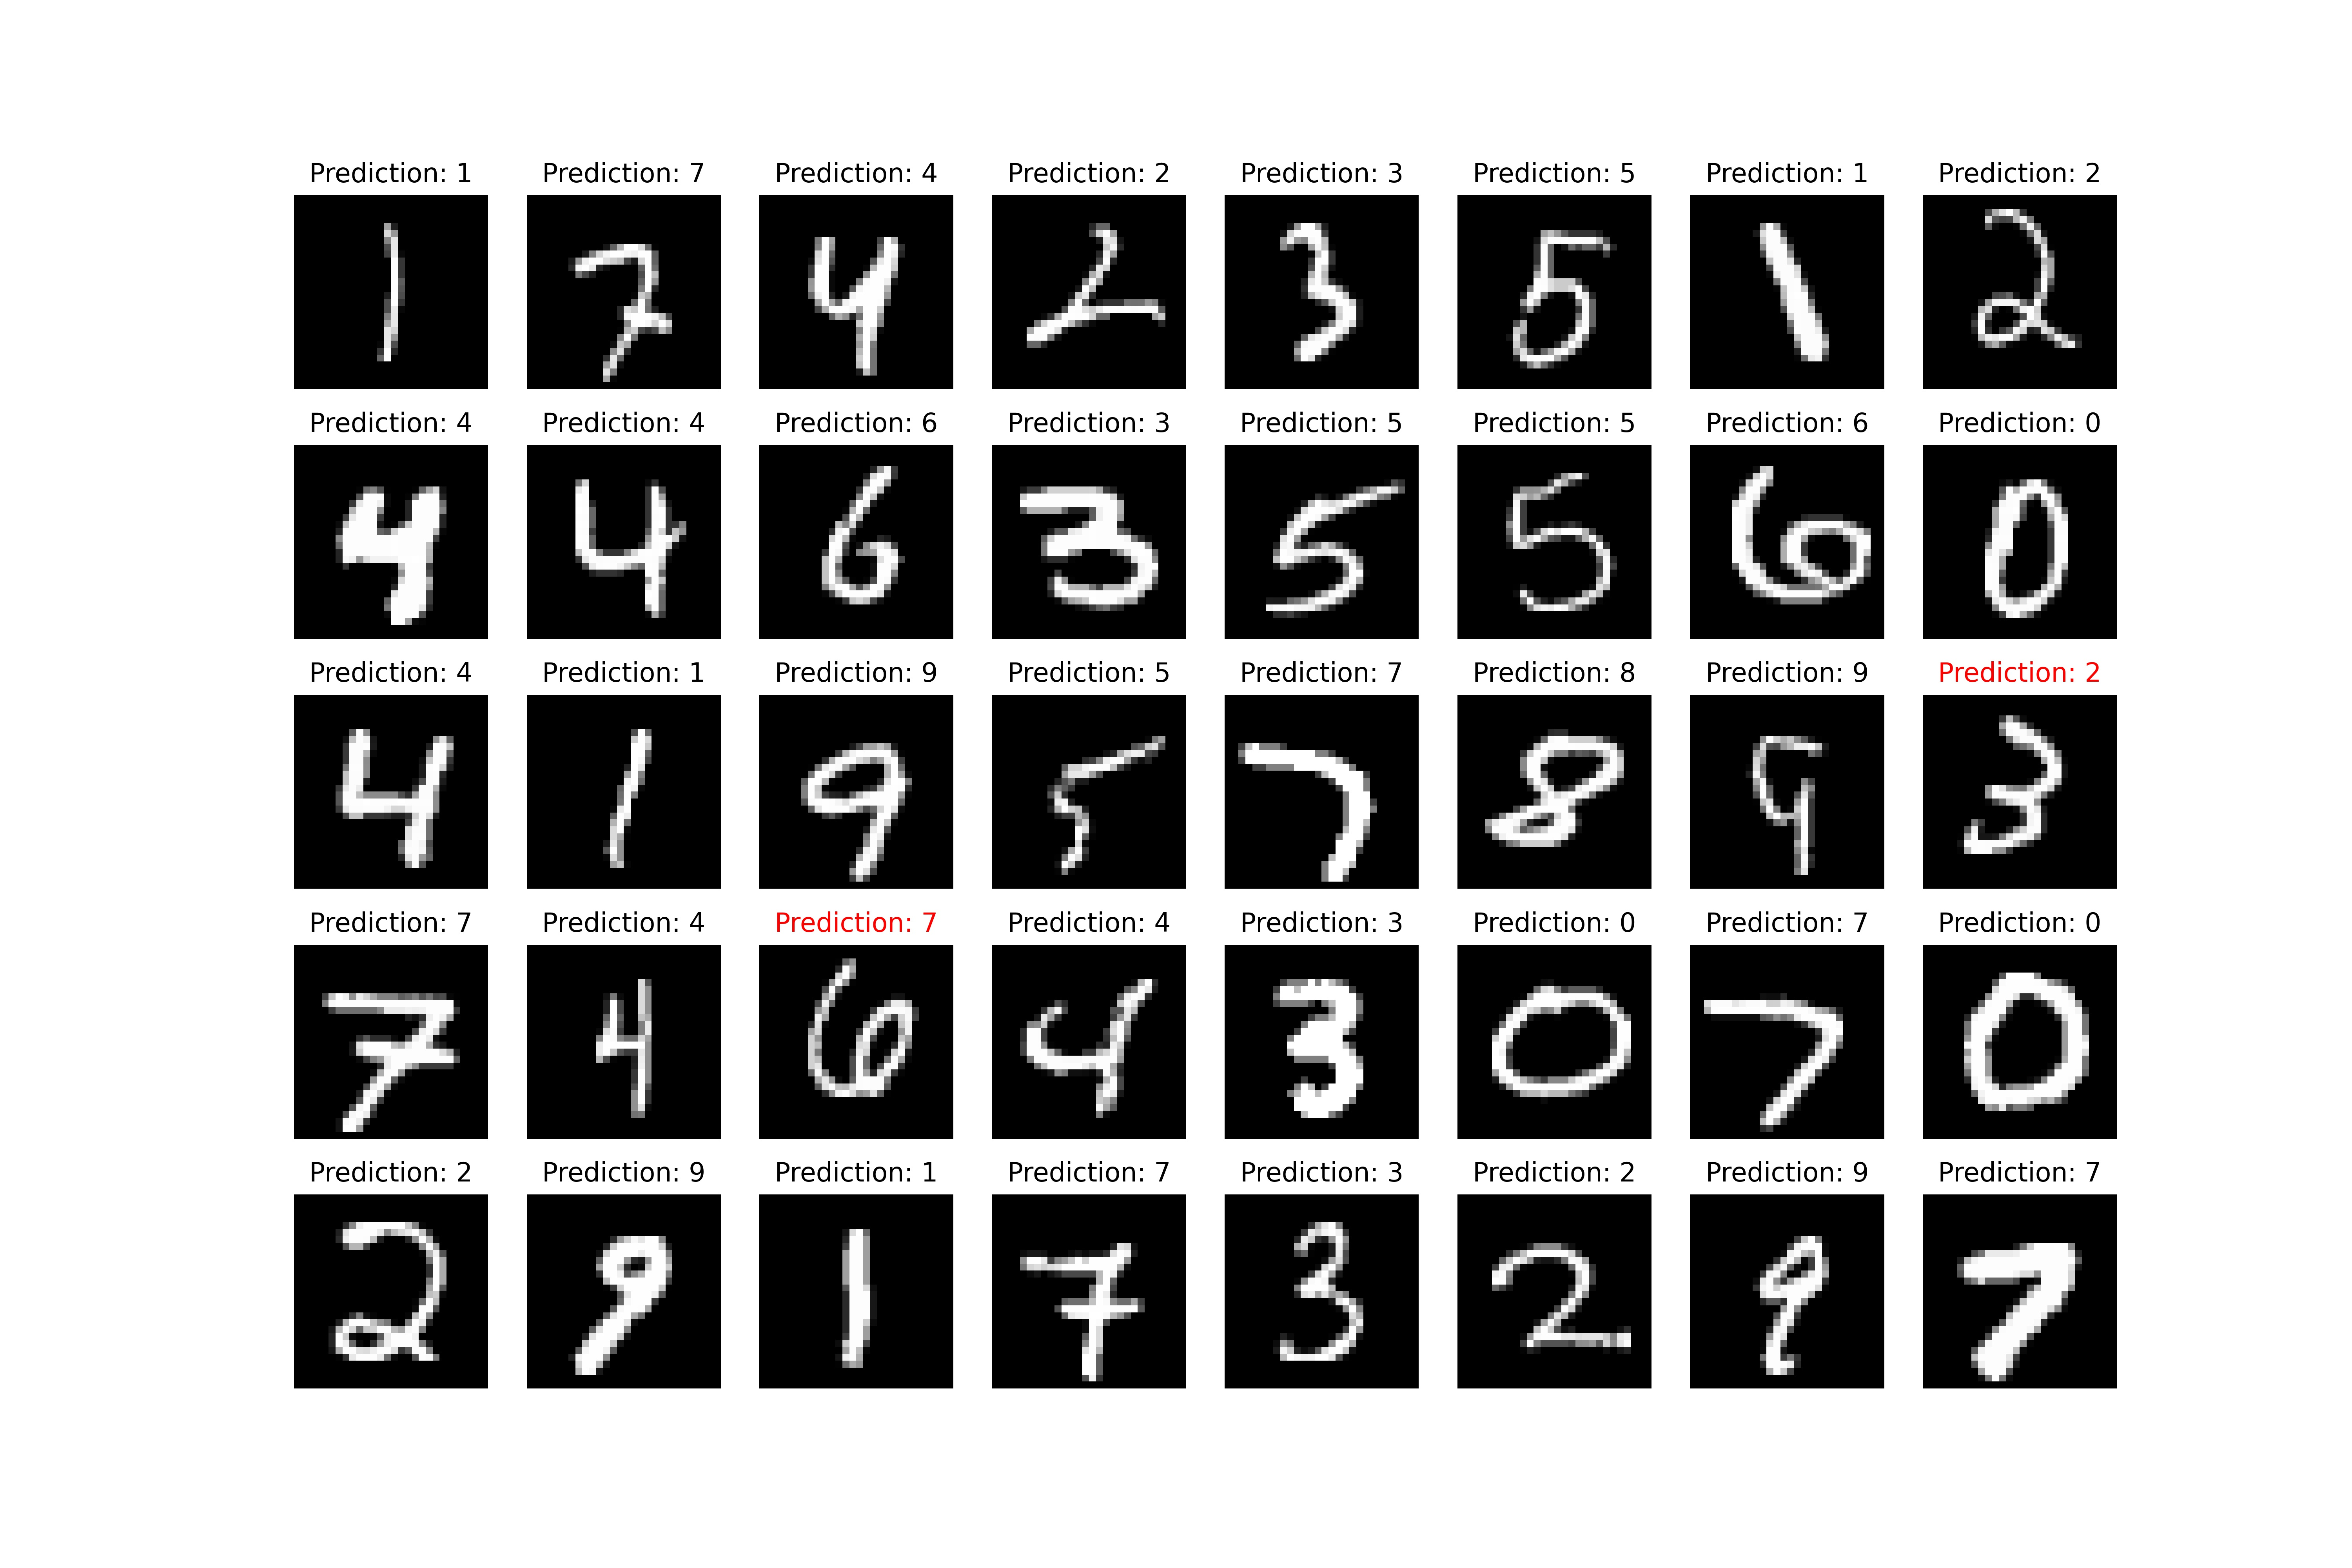
\includegraphics[height=170px]{4-Resultat.jpg}
		\caption{Exemple sur un échantillon de 40 images de validation}
	\end{figure}
\end{frame}

